~\vspace{2em}
\begin{questions}

  \question 一弹簧自然长度为$ l _ { 0 } $,倔强系数为$ k $,将弹簧竖挂,下端垂
  % 219.jpg
  以重物$ m $,重物将弹簧在弹性限度内拉长到一个新的平衡长度$ l _ { 0 } $。
  试问:对于这个新的平衡位置的位移,此弹簧是否具有同样的倔
  强系数?

  \question 在图\ref{fig:07.13}\;所示的诸情况中,哪些是简谐振动?哪些不是简
  谐振动?试说明理由。
  \begin{figurex}
    \centering
    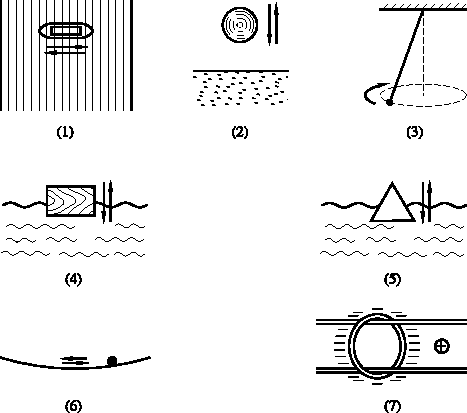
\includegraphics{figure/fig07.13}
    \caption{}
    \label{fig:07.13}
  \end{figurex}

  (1)织布机的梭子置于光滑水平经线上,在两边冲力作用下
  作往返运动;

  (2)小球在光滑水平面上作完全弹性的上下跳动;

  (3)不可伸长的细线悬一小球在水平面上作匀速圆周运动;

  (4)一均匀矩形木块浮在水上,用力将它部分按入水中,然
  后松手,木块作上下浮动,不计水的粘滞阻力;

  (5)在(4)中,换了一个密度小于水的均匀正三棱锥,锥顶向
  上,在水中上下浮动且幅度较大;

  % 220.jpg
  (6)小球在半径很大的较光滑凹球面底部作短距离的往返滚
  动时,球心的运动;

  (7)一个带负电荷的圆环套在水平的光滑薄玻璃管上,玻璃
  管内有一带正电荷的小球,在静电力的作用下作往返运动,假定
  生运动过程中小球和圆环上的电荷分布都不变。

  \question 一个倔强系数为$ k $的弹簧和一质量为$ m $的物体组成一振动
  系统。若弹簧的质量不计,弹簧的自然长度为$ l _ { 0 } $,在下述各情况
  下,振动周期及平衡时弹簧的长度有何不同?

  (1)整个系统放在光滑水平面上,一端固定;

  (2)整个系统竖直挂起;

  (3)整个系统放在倾角为$ \alpha $,光滑斜面上,上端固定。

  \question 两个倔强系数都为$ k $的轻弹簧与一重物$ m $组成以下各种振
  力系统,试问:哪些是简谐振动?如是,则求其周期(图\ref{fig:07.14})。
  \begin{figurex}
    \centering
    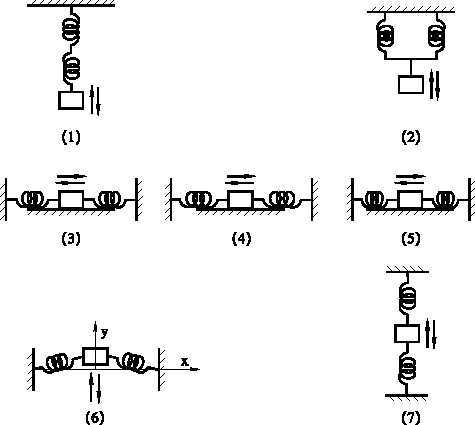
\includegraphics{figure/fig07.14}
    \caption{}
    \label{fig:07.14}
  \end{figurex}

  % 221.jpg
  \clearpage
  (1)串联后,吊起$ m $;

  (2)开联后,吊起$ m $;

  (3)\;$ m $与两弹簧都平放于光滑水平面上,平衡时弹簧处于自
  然状态,$ m $振动方向与弹簧伸长方向相同;

  (4)如(3)放置,但在平衡位置时每个弹簧伸长了$ x _ 0 $;

  (5)如(3)放置,但在平衡位置时每个弹簧压缩了$ x _ 0 $;

  (6)\;$ k $与$ m $放于水平光滑桌面上,$ m $在$ y $方向振动,振动时保
  持两个弹簧长度相等,平衡时两弹簧自然伸长;

  (7)系统竖挂,$ m $在平衡位置时,上面弹簧的伸长量等于下面
  弹簧的缩短量。

  \question 秋千的摆动幅度由大到小时,它的频率会发生什么变化?

  \question 单摆的振幅不是很小时,试证明周期的一般表达式是
  {\setlength{\mathindent}{4em}
  \begin{equation*}
    T = 2 \uppi \sqrt { \frac { l } { g } } \left( 1 + \frac { 1 } { 2 ^ { 2 } } \sin ^ { 2 } \frac { \theta _ { m } } { 2 } + \frac { 1 } { 2 ^ { 2 } } \cdot \frac { 3 ^ { 2 } } { 4 ^ { 2 } } \sin ^ { 4 } \frac { \theta _ { m } } { 2 } + \cdots \right)
  \end{equation*}}
  式中$ \theta _ { m } $是最大角位移。

  \question 如果将单摆、质点-弹簧系统放到月球上去,它们的振动
  频率改变吗?在宇宙飞船上用什么方法测质量?

  \question 一个无质量、长$ l _ { 0 } $、倔强系数为$ k $的弹簧竖直挂在天花板
  上,现将一质量为$ m $的质点挂于弹簧之下。若已知$ m g = k \Delta l $,是否有
  $ m g \Delta l = \dfrac { 1 } { 2 } k \left( \Delta l \right) ^ { 2 } $
  ?为什么?引力作的功是否等于弹簧弹性势
  能的增加量?引力的存在是否会改变这个系统的振动频率、平衡
  位置及总能量?

  \question 一质点受指向原点的力$ F = - 6 x ^ { 3 } $的作用。试问:这质点是
  否作周期运动?这运动是否是简谐振动?

\end{questions}